\chapter{vim编辑器}
\label{sec:vimUsage}

当我们基本熟悉了操作系统的使用,是不是还少了什么件事?恭喜你猜对了,那
就是在系统里面编辑一些东西,我们总该留点什么东西吧,你说是不是呢?

传说中,蔚蓝的星球上流传着两大神器,一个是vi\footnote{vim是vi的升级版,
  一般认为vi\index{vi编辑器}既vim\index{vim编辑器},vim既vi。也可理解为
  vi为vim的一个别名。},一个是emacs。据说Vim是编辑器之神,而Emacs是神的
编辑器。追求独步天下的高手和低手们争着一睹它们的风采,可看到它们朴素单
薄的界面后,不禁心下怀疑:这就是神器吗?至有人生了轻视之心。

本文就向你展示如何使用vim,掌握它最基本的使用即可。作者刚开始使用vim的
时候,总是不由自主地想动动旁边的鼠标,大概用了两个晚上的时间才熟练的掌
握。Emacs可以根据自己兴趣看一看,作者使用了一年多的时间,也没觉得自己比
那些使用vim的家伙强\footnote{这里作者并不想卷入编辑器之战,不想得罪任何
  一方阵营,两种编辑器我都会使用,上班时用vi,不上班时用Emacs;如果真的
  得罪了某方阵营,请原谅我的无知。},我的vi用的比Emacs要熟练。嘿嘿!

\section{vim的几种模式}
\label{sec:vimMode}

vim有两种模式,一个为输入模式,一个为命令模式。在系统提示字
符(如\$、\#)下敲入vim filename,如果没有filename这个文件则会创建,若有则
打开。vim可以自动帮你载入所要编辑的文件或是开启一个新文件(如果该文件不
存在或缺少文件名)。进入vim后屏幕左方会出现波浪符号,凡是列首有该符号就
代表此列目前是空的。

如上所述,vim存在两种模式:指令模式和输入模式。在指令模式下输入的按键将
做为指令来处理:如输入i,vim即认为是在当前位置插入字符。而在输入模式
下,vim则把输入的按键当作插入的字符来处理。指令模式切换到输入模式只需键
入相应的输入命令即可(如a,A),而要从输入模式切换到指令模式,则需在输
入模式下键入ESC键,如果不晓得现在是处于什么模式,可以多按几次ESC,系统
如发出哔哔声就表示已处于指令模式下了。

\subsection{输入模式}

如何进入输入模式?下面列出几个进入插入模式的指令:

\begin{table}[h]
  \centering
    \begin{tabular}{cl}
      \toprule
      指令  & 说明 \\
      \midrule
      i     & 在光标所在处进入插入模式 \\
      I     & 在当前行的行首进入插入模式 \\
      a     & 在光标的后面进入插入模式 \\
      A     & 在当前行的行尾进行插入模式 \\
      o     & 在光标所在行的下面新开一行 \\
      O     & 在光标所在行的上面新开一行 \\
      s     & 删除光标所在字符并进入插入模式 \\
      S     & 删除光标所在行并进入输入模式 \\
      \bottomrule
    \end{tabular}
    \caption{vim进入插入模式指令}
    \label{tab:vimInsertMode}
\end{table}

大家注意到了没有,大写与小写分别控制反向与正向。如何退出呢?在插入模式
下,需要按下键盘的ESC键,进入命令模式,再从命令模式下,输入”:wq“即可
退出。wq的意思是保存并退出,如果不想保存,只需输入”:q“即可。如果修改
后,发现改错了文件,并不想保存了,在命令模式下输入”:q!“即可,加
上”!“作用是强制退出不保存,其实也可以强制保存并退出的,该怎么输入?想
想看。

\subsection{命令模式}

在刚打开vim编辑器时,这时所处的模式是命令模式;从输入模式返回到命令模式,
只需要按下键盘上的ESC键即可返回到命令模式。下面介绍几组很实用的指令,主
要涉及删除、复制及粘贴的指令,还有几个控制光标移动的指令。

光标方向控制:

\begin{table}[h]
  \centering
    \begin{tabular}{cl}
      \toprule
      指令  & 说明 \\
      \midrule
      h    & 光标向前移动 \\
      j  & 光标向下移动 \\
      k  & 光标向上移动 \\
      l  & 光标想后移动 \\
      G  & 按下shift与G组合,则跳到文件末尾 \\
      gg & 连续按两次G,跳到文件的首行 \\
      \bottomrule
    \end{tabular}
    \caption{vim方向控制键}
    \label{tab:vimFangxiang}
\end{table}

撤销指令:

\begin{table}[h]
  \begin{center}
    \begin{tabular}{cl}
      \hline
      指令  & 说明 \\
      \hline
      u    & 按一次,撤销上一次的操作,按两次呢?哈哈 \\
      \hline
      :e!  & 直接回到了刚打开时的状态 \\
      \hline
    \end{tabular}
  \end{center}
\end{table}

删除指令:

\begin{table}[h]
  \begin{center}
    \begin{tabular}{cl}
      \hline
      指令   & 说明 \\
      \hline
      dd    & 删除当前光标所在行 \\
      \hline
      ndd   & 删除当前光标所在行及以下行共n行,其中n为数字 \\
      \hline
    \end{tabular}
  \end{center}
\end{table}

\subsection{vim的其他一些指令}

\section{vim的一些小技巧}

\begin{verbatim}
# 打开文件定位到指定行
vim +24 file       

# 打开多个文件	
vim file1 file2    

# 垂直分屏
vim -O file1 file2 

# 水平分屏
vim -o file1 file2 

# 上下分割打开新文件
sp filename       

# 左右分割打开新文件 
vsp filename      

Ctrl+W [操作]       # 多个文件间操作  大写W  # 操作: 关闭当前窗口c  屏幕高度一样=  增加高度+  移动光标所在屏 右l 左h 上k 下j 中h  下一个w  
:n                 # 编辑下一个文件
:2n                # 编辑下二个文件
:N                 # 编辑前一个文件
:rew               # 回到首文件
:set nu            # 打开行号
:set nonu          # 取消行号
200G               # 跳转到200
:nohl              # 取消高亮
:set autoindent    # 设置自动缩进
:set ff            # 查看文本格式
:set binary        # 改为unix格式
ctrl+ U            # 向前翻页
ctrl+ D            # 向后翻页
% s/字符1/字符2/g   # 全部替换	
X                  # 文档加密
\end{verbatim}

\section{vim复制粘贴及剪切板}

复制粘贴指令:

\begin{table}[!h]
  \begin{center}
    \begin{tabular}{cl}
      \hline
      指令  & 说明 \\
      \hline
      yy    & 复制当前光标所在行 \\
      \hline
      nyy   & 复制当前行及以下行共n行,n为数字 \\
      \hline
      p     & 将复制的内容粘贴到当前光标的下面一行,可以与数字一起使用,如np \\
      \hline
      P     & 将复制的内容粘贴到当前光标的上面一行,可以与数字一起使用,如nP \\
      \hline
    \end{tabular}
  \end{center}
\end{table}

vim有12个粘贴板,分别是0、1、2、...、9、a、“、+;
用:reg命令可以查看各个粘贴板里的内容。效果如图所示:

\begin{figure}[htbp]
  \begin{center}
    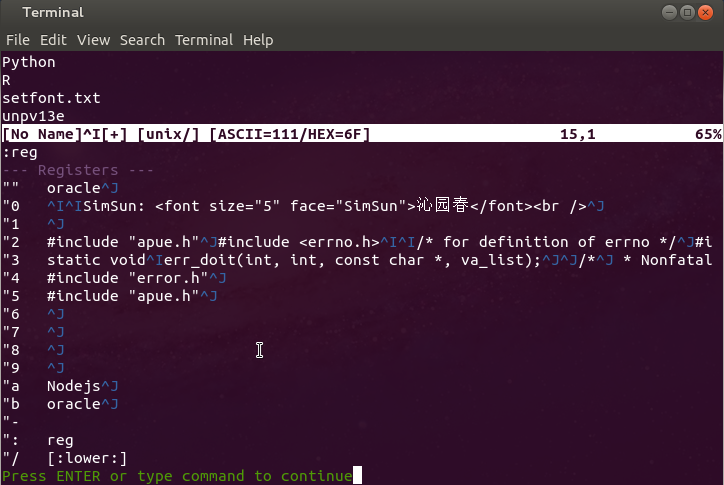
\includegraphics[width=.75\textwidth]{graph/vimregister.png}
  \end{center}
  \caption{vim粘贴板一览}
  \label{fig:vimClipBoard}
\end{figure}

在vim中简单用y只是复制到"(双引号)粘贴板里,同样用p粘贴的内容也是这个
粘贴板里的内容;要将vim的内容复制到某个粘贴板,需要退出编辑模式,进入
正常模式后,选择要将复制的内容,然后按"Ny(注意带引号)完成复制,其中N为
粘贴板号(注意是按一下双引号后按粘贴板号再按y),比如要把内容复制到粘贴
板a,选中内容后按"ay就可以了。

有两点需要说明一下:"号粘贴板(临时粘贴板)比较特殊,直接按y就复制到这个
粘贴板中了,直接按p就粘贴这个粘贴板中的内容;+号粘贴板是系统粘贴板,
用"+y将内容复制到该粘贴板后可以使用Ctrl+V将其粘贴到其他文
档(如firefox、gedit)中,同理,要把在其他地方用Ctrl+C或右键复制的内容复
制到vim中,需要在正常模式下按"+p;

\section{vim配置文件}

我相信,每个有想法的家伙肯定不会满足默认的配置,他们总喜欢捣鼓。这个时
候我们就可以定制自己的编辑器了,以满足我们日常编辑的需求。Emacs的定制配
置更是令人蛋疼,诸多选项、诸多值……。作者曾经也是为此事而蛋疼不已,只是
学会了在Emacs里配置\LaTeX\index{\LaTeX}的一些配置项,其它神马的,作者是
一窍不通。

令人蛋疼的事就不多说,我比较喜欢简洁的配置。本人也不会开发,一些简单的
配置就能满足日常需要了,再说这个东东用的也不多。其它高大上的配置东东对
我来说也是浮云。下面是我常用的vim的配置文件,配置如下:

\begin{verbatim}
[root@iLiuc ~]# cat ~/.vimrc
set nocompatible
filetype indent on
filetype plugin on
set tabstop=4
set shiftwidth=4
set autoindent
set cindent
set smartindent
set hlsearch
syntax enable
set dict=/usr/share/dict/words

if has('statusline')
    set laststatus=2

    " Broken down into easily includeable segments
    set statusline=%<%f\            " Filename
    set statusline+=%w%h%m%r        " Options
    set statusline+=\ [%{&ff}/%Y]   " filetype

    " ASCII/Hexadecimal value of under current cursor
    set statusline+=\ [ASCII=\%03.3b/HEX=\%02.2B]

    " Right aligned file nav info
    set statusline+=%=%-14.(%l,%c%V%)\ %p%%
endif
\end{verbatim}

效果如下:

\begin{figure}[htbp]
  \centering
  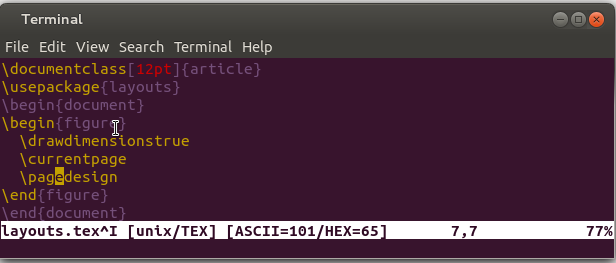
\includegraphics[width=.75\textwidth]{graph/vimrc.png}
  \caption{vim配置文件效果}
  \label{fig:vimConf}
\end{figure}

哦!天呢。根本停不下来了。就说这么多吧,如果我要再写下去,就不止这么多。
呵呵!只不过是两年没用认真的使用了。呵呵!vim的使用就介绍这么多,我想仅
仅学会这些就能让初学者的效率有很大的提高,但还不够高,这里并没有介绍正
则表达式等。
